% !TeX program = pdfLaTeX
\documentclass[aoas]{aoas/imsart}
\usepackage{amsmath,amsfonts,amssymb}
\usepackage{graphicx}
\usepackage[round,sort&compress]{natbib}
\usepackage[letterpaper=true,colorlinks=true,pdfpagemode=none,urlcolor=blue,linkcolor=blue,citecolor=blue,pdfstartview=FitH]{hyperref}
\usepackage{color}
\usepackage{booktabs}


\usepackage{algorithm,algorithmic}
\def\algorithmautorefname{Algorithm}


\renewcommand*{\figureautorefname}{Figure}%
\renewcommand*{\tableautorefname}{Table}%
\renewcommand*{\partautorefname}{Part}%
\renewcommand*{\chapterautorefname}{Chapter}%
\renewcommand*{\sectionautorefname}{Section}%
\renewcommand*{\subsectionautorefname}{Section}%
\renewcommand*{\subsubsectionautorefname}{Section}%



\usepackage{xr}
\externaldocument{aoas/musicManuscript}

%% load any required packages here




% Number only ref'ed equations
\usepackage{mathtools}
\mathtoolsset{showonlyrefs,showmanualtags}

\renewcommand{\algorithmiccomment}[1]{\hfill $\rhd$ #1}
\renewcommand{\thealgorithm}{A\arabic{algorithm}} 

\usepackage{afterpage}

\renewcommand\thefigure{SM-\arabic{figure}}
\newcommand{\email}[1]{\href{mailto:#1}{#1}}

%\usepackage{setspace}

\newcommand{\norm}[1]{\left\lVert #1 \right\rVert}
\renewcommand{\hat}{\widehat}
% next three lines to give Kalman filter sample \varx_t=E[x_t|y_1,...,y_t]
\usepackage{upgreek}
\DeclareRobustCommand{\varx}{{\mathpalette\irchi\relax}}
\newcommand{\irchi}[2]{\protect\raisebox{\depth}{$#1\upchi$}}
\newcommand{\given}{\ \vert\ }
\newcommand{\E}{\mathbb{E}}
\newcommand{\Expect}[1]{\E\left[#1\right]}
\newcommand{\Var}[1]{\mathbb{V}\left[#1\right]}
\newcommand{\indicator}[1]{\boldsymbol{1}\left(#1\right)}

\begin{document}

\begin{frontmatter}
  
\title{Supplement to Markov-Switching State Space Models for Uncovering Musical
  Interpretation}
\runtitle{Supplement to Switching Models for Music}
\author{%
  \fnms{Daniel J.} \snm{McDonald}\corref{}\ead[label=e1]{dajmcdon@indiana.edu}\thanksref{t1}},
\author{%
  \fnms{Michael} \snm{McBride}\ead[label=e2]{michmcbr@iu.edu}},
\author{%
  \fnms{Yupeng} \snm{Gu}\ead[label=e3]{yupeng.gu@gmail.com}},
\and
\author{\fnms{Christopher} \snm{Raphael}\ead[label=e4]{craphael@indiana.edu}\thanksref{t2}}
\thankstext{t1}{DJM was partially supported by 
  the National Science Foundation Grants DMS-1407439
  and DMS-1753171.}
\thankstext{t2}{CR was partially supported by the National Science
  Foundation Grant IIS-1526473.}
\affiliation{Indiana University, Bloomington}
\runauthor{McDonald, McBride, Gu, and Raphael}
\address{Daniel J.\ McDonald and\\Michael McBride\\Department of
  Statistics\\ Myles Brand Hall\\ Bloomington, IN
  47408\\ \printead{e1}\\ \phantom{E-mail:\ }\printead*{e2}}
\address{Yupeng Gu and\\Christopher Raphael\\School of Informatics,
  Computing,\\ and Engineering\\ Myles Brand Hall\\ Bloomington, IN
  47408\\ \printead{e3}\\ \phantom{E-mail:\ }\printead*{e4}}

\end{frontmatter}




\hypertarget{algorithms}{%
\section{Algorithms}\label{algorithms}}

For completeness, we include here concise descriptions of the Kalman
filter and smoother we employ as inputs to our main algorithm. The
filter is given in \autoref{alg:kalman}.

\begin{algorithm}
  \caption{Kalman filter: estimate $x_i$ conditional on
    $\{y_j\}_{j=1}^i$, for all $i=1,\ldots,n$ and calculate the log likelihood
    for $\theta$\label{alg:kalman}}
  \begin{algorithmic}
    \STATE {\bf Input:} $Y$, $x_0$, $P_0$, $d,\ T,\ c,\ Z,$ and $G$
    \STATE $\ell(\theta) \leftarrow 0$ \COMMENT{Initialize the log-likelihood}
    \FOR{$i=1$ to  $n$}
    \STATE $\begin{aligned}\varx_{i}
      &\leftarrow d + T x_{i-1|i-1}, & P_i &\leftarrow Q + T P_{i-1|i-1}
      T^\top\end{aligned}$ \COMMENT{Predict current state}
    \STATE $\begin{aligned}\widetilde{y}_i
      &\leftarrow c + Z \varx_i, & F_i &\leftarrow G + Z P_i
      Z^\top\end{aligned}$ \COMMENT{Predict current observation}
    \STATE $\begin{aligned}v_i&\leftarrow y_i-\widetilde{y}_i& K_i&
      \leftarrow P_i Z^\top F^{-1}\end{aligned}$ \COMMENT{Forecast error and 
    Kalman gain}
    \STATE $\begin{aligned} x_{i|i}
      &\leftarrow \varx_i + K_i v_i, & P_{i|i} &\leftarrow P_i - P_iZ^\top
      K_i\end{aligned}$ \COMMENT{Update}
    \STATE $\ell(\theta) = \ell(\theta) -v_i^\top F^{-1}v_i - \log(|F_i|)$
    \ENDFOR
    \RETURN $\widetilde{Y}=\{\widetilde{y}_i\}_{i=1}^n,\ \varx=\{\varx_i\}_{i=1}^n,\
    \widetilde{X}=\{x_{i|i}\}_{i=1}^n,\ P=\{P_i\}_{i=1}^n,\
    \widetilde{P}=\{P_{i|i}\}_{i=1}^n,\ \ell(\theta)$
  \end{algorithmic}
\end{algorithm}

To incorporate all future observations into these estimates, the Kalman
smoother is required. There are many different smoother algorithms
tailored for different applications. \autoref{alg:kalman-smoother}, due
to \citet{RauchStriebel1965}, is often referred to as the classical
fixed-interval smoother \citep{AndersonMoore1979}. It produces only the
unconditional expectations of the hidden state
\(\hat{x}_i=\Expect{x_i\given y_1,\ldots,y_n}\) for the sake of
computational speed. This version is more appropriate for inference in
the type of switching models we discuss in the manuscript.

\begin{algorithm}
  \caption{Kalman smoother (Rauch-Tung-Striebel): estimate $\hat{X}$ conditional on
    $Y$\label{alg:kalman-smoother}} 
  \begin{algorithmic}
    \STATE {\bf Input:} $\varx$, $\widetilde{X}$, $P$, $\widetilde{P}$,
    $T,$ $c$, $Z$.
    \STATE $t=n$,
    \STATE $\hat{x}_{n}\leftarrow \widetilde{x}_n$, 
    \WHILE{$t>1$}
    \STATE $\hat{y}_i \leftarrow c + Z\hat{x}_i,$
    \COMMENT{Predict observation vector}
    \STATE $\begin{aligned} e &\leftarrow \hat{x}_i -
      \varx_i, & V &\leftarrow P_i^{-1}\end{aligned}$,
    \STATE $t\leftarrow i-1$, \COMMENT{Increment}
    \STATE $\hat{x}_i = \widetilde{x}_i + \widetilde{P}_i T Ve $ 
    \ENDWHILE
    \RETURN $\widehat{Y}=\{\hat{y}_i\}_{i=1}^n, \hat{X}=\{\hat{x}_i\}_{i=1}^n$
  \end{algorithmic}
\end{algorithm}

\hypertarget{distance-matrix-from-raw-data}{%
\section{Distance matrix from raw
data}\label{distance-matrix-from-raw-data}}

In \autoref{sec:clust-music-perf} of the manuscript, we present results
for clustering performances using the low-dimensional vector of
performance specific parameters learned for our model. An alternative
approach is to simply use the raw data, in this case, 231 individual
note-by-note instantaneous speeds measured in beats per minute. In
\autoref{fig:raw-data-clusters} we show the result of this analysis. A
comparison between this clustering and that given by our model is
discussed in some detail in the manuscript.

\begin{figure}[b]

{\centering 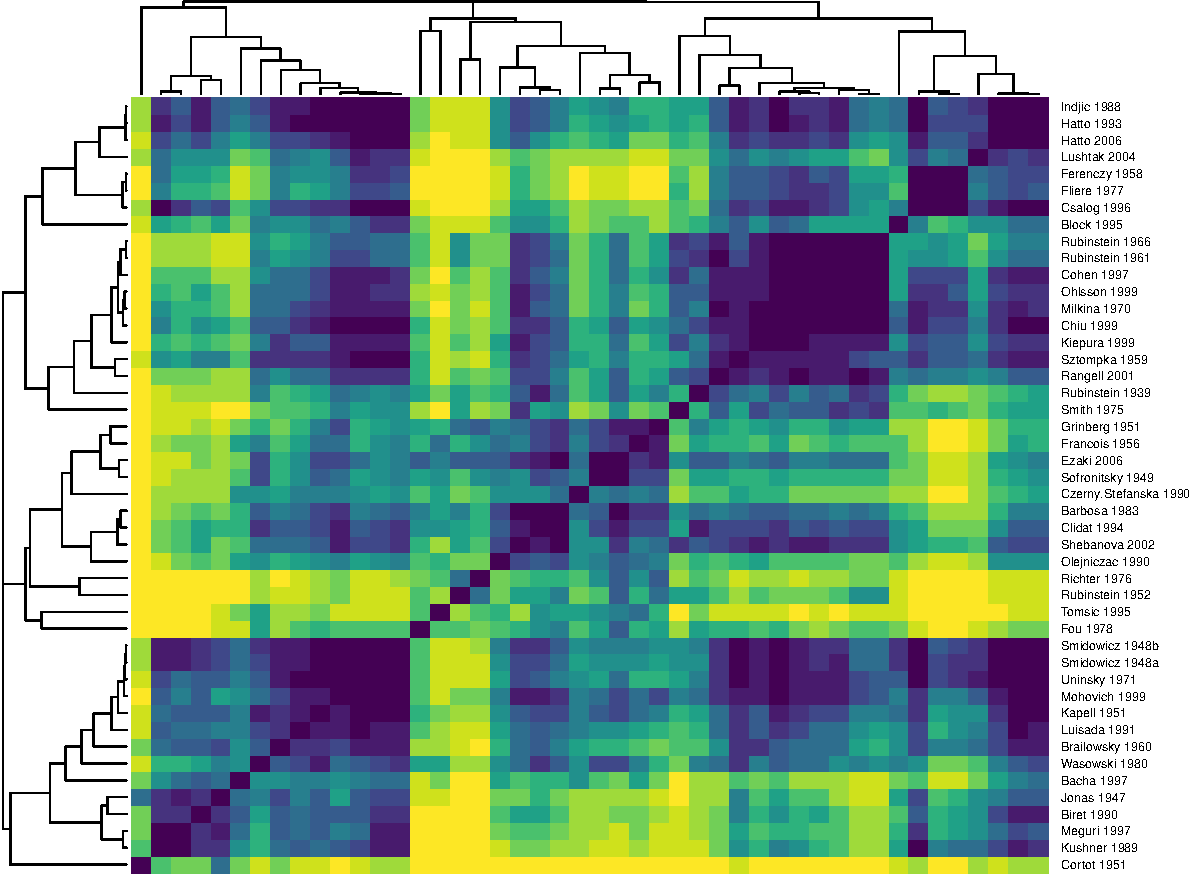
\includegraphics[width=3in,height=3in]{gfx/raw-data-clusters-1} 

}

\caption{This figure presents a heatmap and hierarchical clustering based only on the note-by-note onset timings for each of the 46 recordings.}\label{fig:raw-data-clusters}
\end{figure}

\hypertarget{plotting-performances}{%
\section{Plotting performances}\label{plotting-performances}}

\autoref{sec:clust-music-perf} of the manuscript discusses 4 distinct
clusters of the 46 performances as well as an ``other'' category of
relatively unique interpretations. Figures \ref{fig:clust-1} to
\ref{fig:clust-other} display the note-by-note tempos along with the
inferred interpretive decisions for all performances by clustering. Here
we include some of the discussion of these clusters from the main text
to clarify the figures.

The first cluster (\autoref{fig:clust-1}) corresponds to performances
which are reasonably staid. The emphasis state is rarely visited with
the performer tending to stay in the constant tempo state with periods
of slowing down at the ends of phrases. Acceleration is never used. Such
state preferences are clearly inferred by the model as shown in, e.g.,
the top row of \autoref{fig:clust-density-tp}. Furthermore, these
performances have relatively low average tempos, and not much difference
between the A and B sections.

\begin{figure}

{\centering 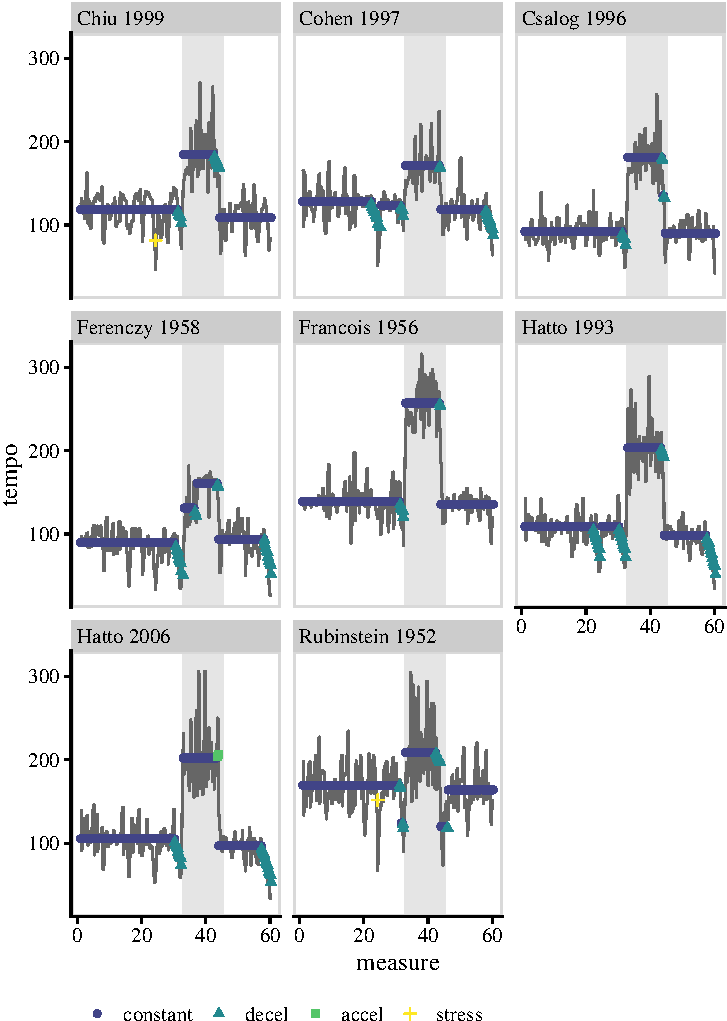
\includegraphics{gfx/clust-1-1} 

}

\caption{Performances in the first cluster.}\label{fig:clust-1}
\end{figure}

Recordings in the second cluster (\autoref{fig:clust-2}) tend to
transition quickly between states, especially constant tempo and slowing
down accompanied by frequent transitory emphases. The probability of
remaining in state 1 is the lowest for this cluster while the
probability of entering state 2 from state 1 is the highest. The
acceleration state is visited only rarely.

\begin{figure}

{\centering 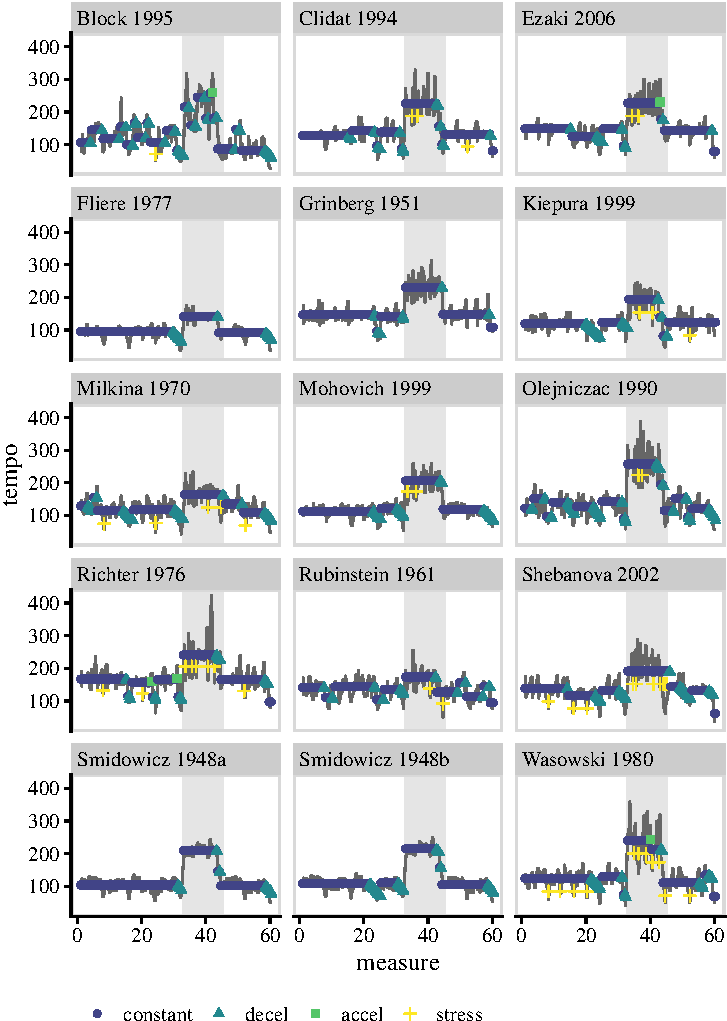
\includegraphics{gfx/clust-2-1} 

}

\caption{Performances in the second cluster.}\label{fig:clust-2}
\end{figure}

Cluster three (\autoref{fig:clust-3}) is somewhat like cluster one in
that performers tend to stay in state 1 for long periods of time, but
they transition more quickly from state 3 back to state 1. They also use
state 4 frequently whereas cluster one did not. They also tend to have
very large tempo contrasts between the A and B sections.

\begin{figure}

{\centering 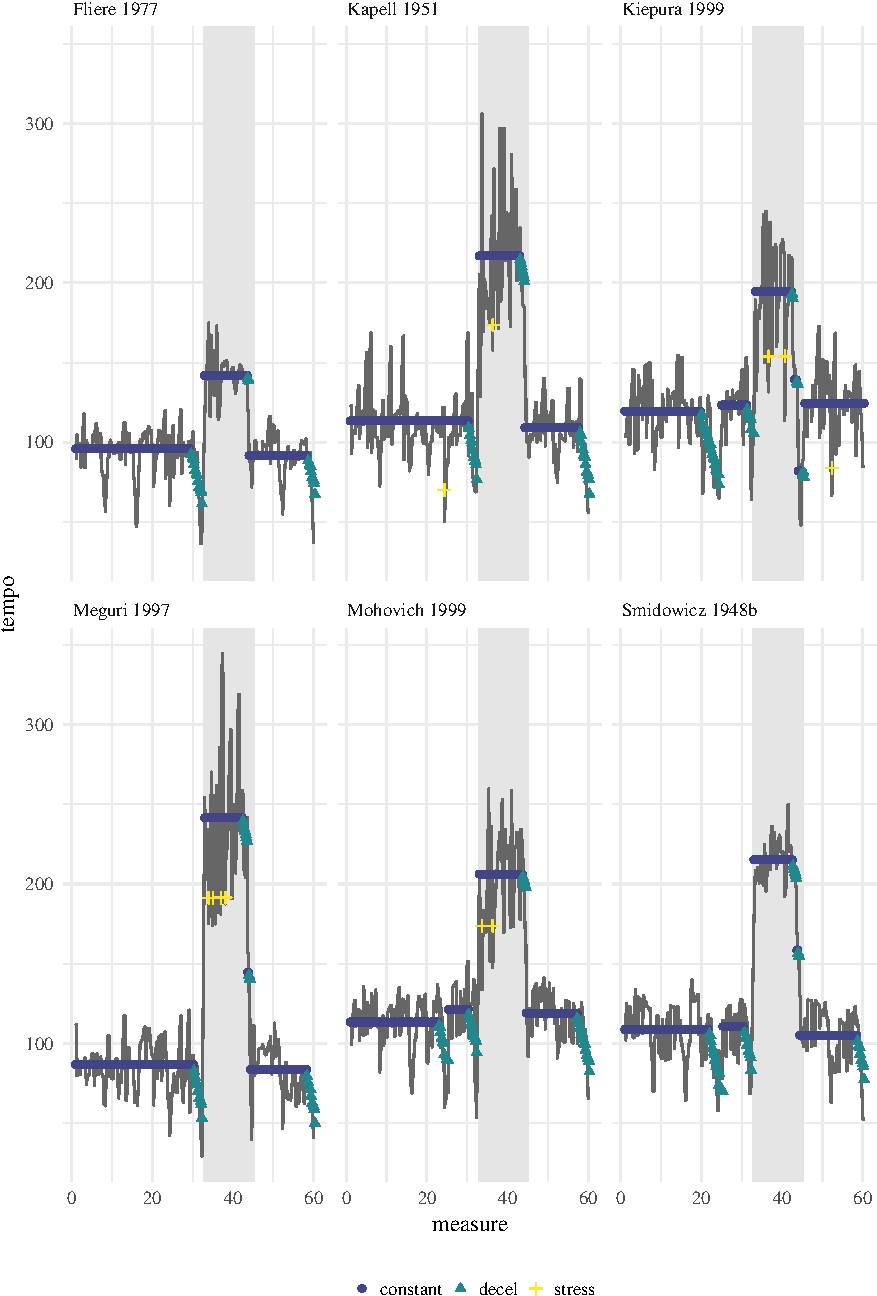
\includegraphics{gfx/clust-3-1} 

}

\caption{Performances in the third cluster.}\label{fig:clust-3}
\end{figure}

Cluster four (\autoref{fig:clust-4}) has both faster average tempos and
more variability from one period of constant tempo to the next. State 4
is rare, with fast constant tempo changes that persist for small amounts
of time tending to reflect note emphases.

\begin{figure}

{\centering 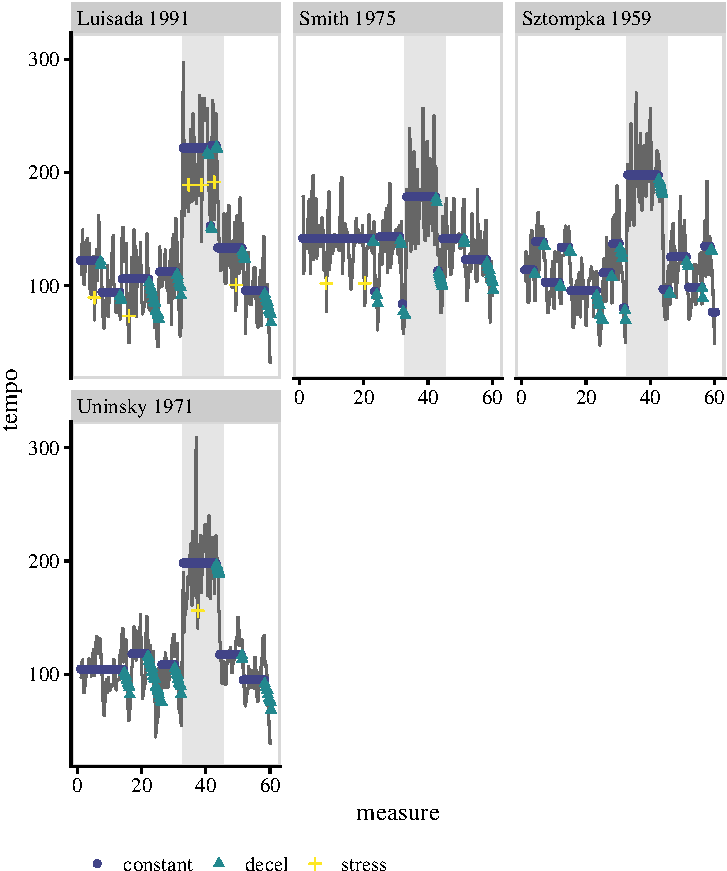
\includegraphics{gfx/clust-4-1} 

}

\caption{Performances in the fourth cluster.}\label{fig:clust-4}
\end{figure}

The remaining performances are relatively different from all other
performances (\autoref{fig:clust-other}). If the distance to the third
closest performances exceeded 0.4, then the performance was grouped with
``other''. Essentially, these recordings had at most one similar
recording while the four other clusters contained at least 3.

\begin{figure}

{\centering 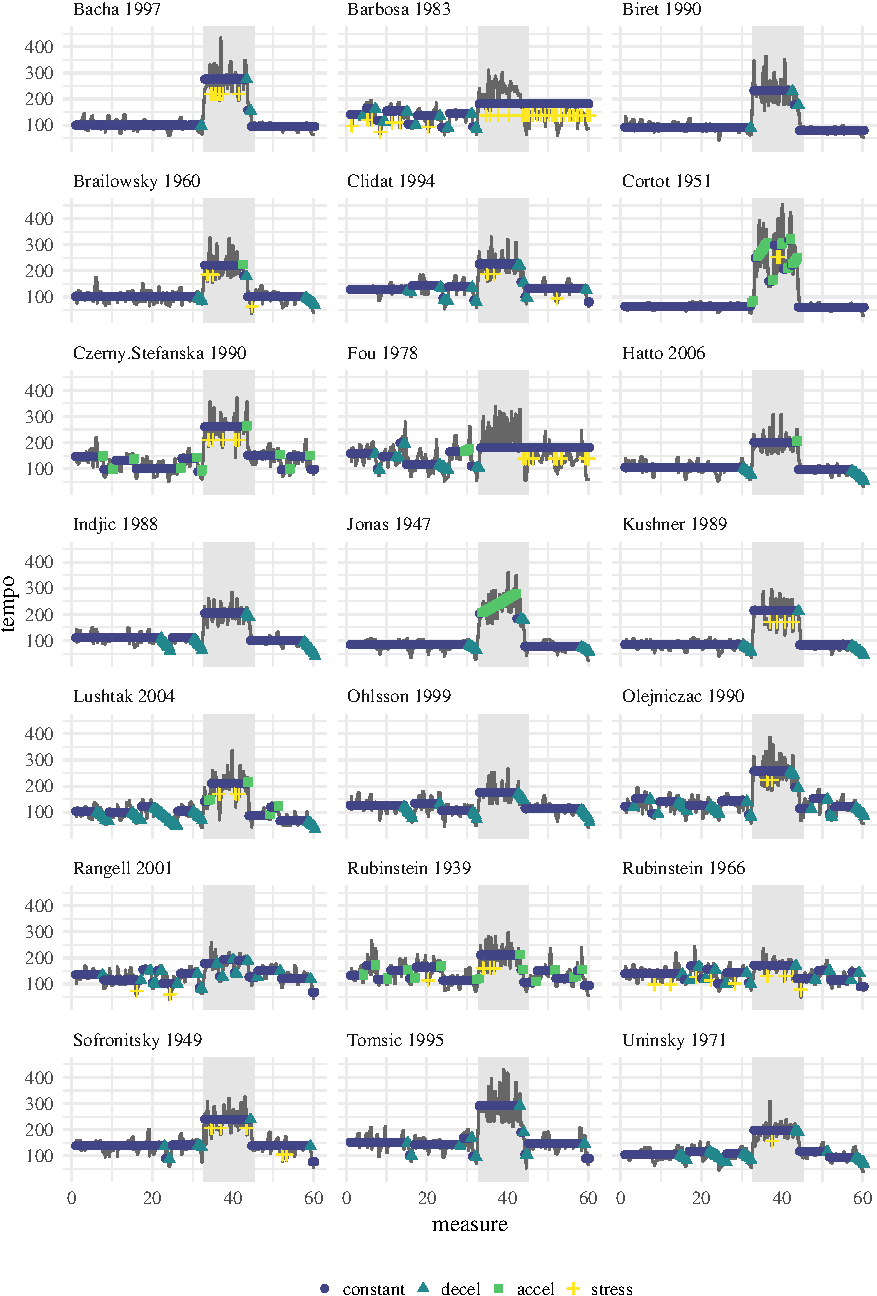
\includegraphics{gfx/clust-other-1} 

}

\caption{Performances in the ``other'' cluster.}\label{fig:clust-other}
\end{figure}

\hypertarget{distribution-over-states}{%
\section{Distribution over states}\label{distribution-over-states}}

To examine the stability of the \autoref{alg:dpf}, we examined all the
potential paths for Richter's 1976 recording. Here, we saved the most
likely 10,000 paths and their weights (rather than only the most likely
path). \autoref{fig:posterior-richter-plot} shows the marginal
(posterior) probability of being in a particular state for each note.
While the paper uses the most likely \emph{path}, this figure is
marginal in the sense that a particular note/state combination may have
high probability in that many paths visited that note/state. But, the
most likely path may not have used that same note/state combination.
Nonetheless, there appears to be consensus for many of the notes. The
most obviously difficult notes are those near measures 10 and 50. In
both cases, the most likely path (\autoref{fig:richter} in the main
text) used the stress state, which exceeds 50\% posterior probability
here.

\begin{figure}

{\centering 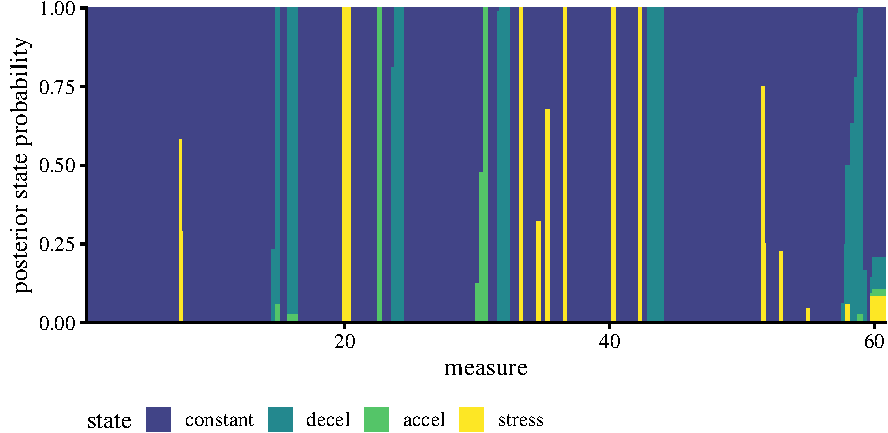
\includegraphics[height=2in]{gfx/posterior-richter-plot-1} 

}

\caption{Distribution over potentitial states for Richter's 1976 recording.}\label{fig:posterior-richter-plot}
\end{figure}


\clearpage

\bibliographystyle{mybibsty}
\bibliography{chopinrefs.bib}

\end{document}
